\documentclass[14pt]{article}
\usepackage[utf8]{inputenc}

\usepackage{algorithm}
\usepackage{algpseudocode}

\usepackage{graphicx}   % LaTex packasge to import graphics.
\graphicspath{{images/}}

\usepackage{amsmath}
\numberwithin{equation}{subsection}

\title{Genetic Algorithms}
\author{Mohamed Mahmoud Mohamed Ahmed}
\date{January 2023}

\begin{document}

\maketitle

\newpage

\section{Introduction}
Evolutionary algorithms (EAs) are the most influential metaheuristics 
for optimization. Genetic Algorithm (GA) is the most popular form of EA. In this article, we first give an introduction to evolutionary computation. 
A state-of-the-art description of GA is then presented.
    \subsection{Introduction to Evolutionary Computation}
    Evolutionary algorithms (EAs) are a class of general-purpose stochastic global optimization algorithms under
		the universally accepted neo-Darwinian paradigm for simulating the natural evolution of biological systems.
		The neo-Darwinian paradigm is a combination of classical Darwinian evolutionary theory, the electionism of
		Weismann, and the genetics of Mendel. Evolution itself can be accelerated by integrating learning, either in
		the form of the Lamarckian strategy or based on the Baldwin effect. EAs are currently a major approach to
		adaptation and optimization. EAs and similar population-based methods are simple, parallel, general-purpose,
		global optimization methods. They are useful for any optimization problem, particularly when conventional
		calculus-based optimization techniques are difficult to implement or is inapplicable. EAs can reliably solve
		hard problems fast that are large, complex, noncontinuous, nondifferentiable, and multimodal. The approach is
		easy to hybridize, and can be directly interfaced to existing simulations and models. EAs can always reach
		the near-optimum or the global maximum. EAs possess inherent parallelism by evaluating multipoints
		simultaneously. A typical EA may consist of a population generator and selector, a fitness estimator, and
		three basic genetic operators, namely, crossover(also called recombination), mutation, and selection.
		Individuals in a population compete and exchange information with one another. Biologically, both crossover
		and mutation are considered the driving forces of evolution. Crossover occurs when two parent chromosomes,
		normally two mologous instances of the same chromosome, break and then reconnect but to the different end
		pieces. Mutations can be caused by copying errors in the genetic material during cell division and by
		external environment factors. Although the overwhelming majority of mutations have no real effect, some can
		cause disease in organisms due to partially or fully nonfunctional proteins arising from the errors in the
		protein sequence. The procedure of a typical EA (in the form of GA) is given by Algorithm 1. The initial
		population is usually generated randomly, while the population of other generations are generated from some
		selection/reproduction procedure. The search process of an EA will terminate when a termination criterion is
		met. Otherwise a new generation will be produced and the search process continues. The termination criterion
		can be selected as a maximum number of generations, or the convergence of the genotypes of the individuals.
		Convergence of the genotypes occurs when all the values in the same positions of all the strings are
		identical, and crossover has no effect for further processes. Phenotypic   onvergence without genotypic
		convergence is also possible. For a given system, the objective values are required to be mapped into fitness
		values so that the domain of the fitness function is ways greater than zero.
    \begin{algorithm}
    \caption{(EA)} % $\label{}
    \begin{enumerate}
        \item Set t = 0.
        \item Randomize initial population $p (0)$.
        \item \textbf{Repeat}:
            \begin{itemize}
                \begin{enumerate}
									\item Evaluate fitness of each individual of $P(t)$.
									\item Select individuals as parents from $P(t)$ based on fitness.
									\item Apply search operators (crossover and mutation) to parents, and generate $P(t + 1)$.
									\item Set $t = t + 1$.
									\item[] \textbf{until} termination criterion is satisfied
								\end{enumerate}
            \end{itemize}
    \end{enumerate}
    \end{algorithm}\par
		EAs are directed stochastic global search. They employ a structured, yet randomized, parallel multipoint
		search strategy that is biased toward reinforcing search
		points of high fitness. The evaluation function must be calculated for all the individuals of the population,
		thus resulting in a high computation load. The high computational cost can be reduced by introducing learning
		into EAs, depending on the prior
		knowledge of a given optimization problem.
		EAs can be broadly divided into genetic algorithms (GAs) , evolution
		strategies (ESs), evolutionary programming, genetic programming (GP)
		differential evolution (DE), and estimation of distribution algorithms
		(EDAs).
		\subsection{Terminologies of Evolutionary Computation}
		Some terminologies that are used in the evolutionary computation literature are listed
		below. These terminologies are an analogy to their biological counterparts. \vspace{1mm}
		
		\noindent \textbf{Definition 1.1 (Population).} A set of individuals in a generation is called a population, 
		P(t) = x1, x2, . . . , xNP, where xi is the ith individual and NP is the size of the population. \vspace{2mm}
		
		\noindent \textbf{Definition 1.2 (Chromosome).} Each individual xi in a population is a single chromosome. A
		chromosome, sometimes called a genome, is a set of parameters that define a solution to the problem. \vspace{2mm}
		
		\noindent \textbf{Definition 1.3 (Gene).}In EAs, each chromosome x comprises of a string of elements xi,
		called genes,	i.e., x = (x1, x2, . . . , xn), where n is the number of genes in the	chromosome. Each gene
		encodes a parameter of the problem into the chromosome. A gene is usually encoded as a binary string or 
		areal number. \vspace{2mm}
			
		\noindent \textbf{Definition 1.4 (Allele).} The biological definition for an allele is any one of a number of
		alternative forms of the same gene occupying a given position called a locus on a chromosome. The gene’s
		position in the chromosome is called locus. \vspace{2mm}
		
		\noindent \textbf{Definition 1.5 (Genotype).}A genotype is biologically referred to the underlying genetic
		coding of a living organism, usually in the form of DNA. In EAs, a genotype represents a coded solution, that
		is, an individual’s chromosome. \vspace{2mm}
			
		\begin{center}
				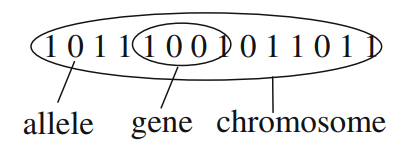
\includegraphics[width=5cm, height=4cm]{Genotype.PNG}
		\end{center}
		
		\noindent \textbf{Definition 1.6 (Phenotype).}Biologically, the phenotype of an organism is either its total
		physical appearance and constitution or a specific manifestation of a trait. There is a phenotype associated
		with each individual. The phenotype of an individual is the set of all its traits (including its fitness and
		its genotype). \vspace{2mm}
		
		\noindent \textbf{Definition 1.7 (Fitness).}Fitness in biology refers to the ability of an individual of
		certain genotype to reproduce. The set of all possible genotypes and their respective fitness values is called
		a fitness landscape. \vspace{2mm}
		
		\noindent \textbf{Definition 1.8 (Natural Selection).}Natural selection alters biological populations over
		timeby propagating heritable traits affecting individual organisms to survive and reproduce. It adapts a
		species to its environment. Natural selection does not distinguish between its two forms, namely, ecological
		selection and sexual selection, but it is concerned with those traits that help individuals to survive the
		environment and to reproduce. Natural selection causes traits to become more prevalent when they contribute to
		fitness. \vspace{2mm}
		
		\noindent \textbf{Definition 1.9 (Genetic Drift).}As opposed to natural selection, genetic drift is a
		stochastic process that arises from random sampling in the reproduction. Genetic drift is the tendency of the
		selection mechanism to converge over time toward auniform distribution of mutants of the fittest individual. It
		changes allele frequencies (gene variations) in a population over many generations and affects traits that are
		more neutral. \vspace{2mm}
		
	\section{Methodologies}
		\subsection{Encoding/Decoding}
		GA uses binary coding. A chromosome x is a potential solution, denoted by a concatenation of the parameters
		x = (x1, x2, . . . , xn), where each xi is a gene, and the value of xi is an allele. x is encoded in the form
		
		\begin{center}
				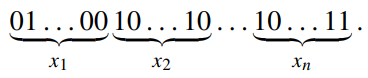
\includegraphics[width=5cm, height=2cm]{encoding-decoding_1.PNG}
		\end{center}
		
		If the chromosome is $l$-bit long, it has $2^l$ possible values. If the variable $xi$ is in the range 
		$[xi−, xi+]$ with	a coding $sli . . . s2s1,$ where $li$ is its bit-length in the chromosome and $si ∈ {0, 1}$, 
		then the decoding function is given by
		
		\[X_i = X_i^- + (X_i^+ - X_i^-)\frac{1}{2^{l_i}-1}(\sum_{j=0}^{l_i-1}{s_j 2^j})\]
		
		In binary coding, there is the so-called Hamming cliffs phenomenon, where large Hamming distances between the
		binary codes of adjacent integers occur. Gray coding is another approach to encoding the parameters into bits.
		The decimal value of a Gray-encoded integer variable increases or decreases by 1 if only one bit is changed.
		However, the Hamming distance does not monotonically increase with the difference in integer values. For a long
		period, Gray encoding was believed to outperform binary encoding in GA. However, based on a Markov chain
		analysis of GA, there is little difference between the performance of binary and Gray codings for all possible
		functions. Also, Gray coding does not necessarily improve the performance for functions that
		have fewer local minima in the Gray representation than in the binary representation. This reiterates the no
		free lunch theorem, namely, no representation is superior for all classes of problems.\par
		
		The performance of GA depends on the choice of the encoding techniques. GA usually uses fixed-length binary
		coding, which results in limited accuracy and slow convergence when approaching the optimum. This drawback can
		also be eliminated by introducing adaptation into GA. Greater accuracy in the final solution is obtained and
		convergence speed is increased by dynamically controlling the coding of the search space. Examples of adaptive
		coding include delta coding, dynamic parameter encoding, and fuzzy coding. There are also
		variable-length encoding methods. In messy GA, both the value and the position of each bit are
		encodedin the chromosome.The addition of fuzzy rules to control coding changes provides a more uniform
		performance in GA search. Examples of fuzzy encoding techniques for GA are the fuzzy GA parameter coding
		and the fuzzy coding for chromosomes. Compared with other coding methods, each parameter in the fuzzy
		coding always falls within the desired range, thus removing the additional overheads on the genetic
		operators. Prior knowledge from the problem domain can be integrated easily.
		
		\subsection{Selection/Reproduction}
		Selection embodies the principle of survival of the fittest, which provides a driving force in GA. Selection is
		based on the fitness of the individuals. From a population $P(t)$, those individuals with strong fitness will
		be selected for reproduction so as to generate a population of the next generation, $P(t + 1)$. Chromosomes with
		larger fitness are selected and are assigned a higher probability of reproduction. Sampling chromosomes from
		the sample space can be in a stochastic manner, a deterministic manner, or their mixed mode. The roulette-wheel
		selection is a stochastic selection method, while the ranking selection and the tournament selection are mixed
		mode selection methods. Other approaches that incorporate mating preferences into evolutionary systems
		are correlative tournament selection and seduction.
		
			\subsubsection{Roulette-Wheel Selection}
			The roulette-wheel or proportional selection is a simple and popular selection scheme. Segments of the
			roulette wheel are allocated to individuals of the population in proportion to the individuals’ relative
			fitness scores. Selection of parents is carried out by successive spins of the roulette wheel, and an
			individual’s possibility of being selected is based on its fitness:

			\[p_i = \frac{f(x_i)}{\sum_{i=1}^{N_p}{f(x_i)}}, \hspace{1cm} i = 1,2,...,N_p\]
			
			
			\noindent Consequently, a chromosome with larger fitness has a possibility of getting more offspring. \par
			Only two chromosomes will be selected to undergo genetic operations. Typically, the population size NP is
			relatively small, and this proportional selection may select a disproportionately large number of unfit
			chromosomes. This easily induces premature convergence when all the individuals in the population become very
			similar after a few generations. GA thus degenerates into a Monte Carlo-type search method.
			
			\subsubsection{Ranking Selection} Ranking selection can eliminate some of the problems inherent in proportional
			selection. It can maintain a more constant selective pressure. Individuals are sorted according to their
			fitness values. The best individual is assigned the maximum rank NP and the worst individual the lowest rank 1.
			The selection probability is linearly assigned according to their ranks
			
			\[P_i = \frac{1}{N_p}(\beta-2(\beta-1)\frac{i-1}{N_p-1}), \hspace{1cm} i = 1,2,...,N_p\]
			
			where $\beta$ is selected in [0, 2].
			
			\subsubsection{Tournament Selection} Tournament selection involves $h$ individuals at a time. The h
			chromosomes are compared and a copy of the best performing individual becomes part of the mating pool. The
			tournament will be performed repeatedly NP times until the mating pool is filled. Typically, the tournament
			size h, which controls the selective pressure, is selected as 2. Tournament selection only uses local
			information. It is very easy to implement in parallel and its time complexity is small. However, tournament
			selection suffers from selection bias, and the best one will not be selected. Unbiased tournament selection
			is suggested to diminish the selective error. Boltzmann tournament selection introduces probability into
			tournament selection. In binary Boltzmann tournament selection, two individuals i and j are picked up
			randomly with replacement. The probability of i winning the tournament is given by 
			$p_i = \frac{1}{1+exp( \frac{f_j-f_i}{T})}$
			 where $T$ is a temperature decreasing as an annealing process, and $f_i$ and $f_j$ are fitness values of
			individual $i$ and $j$, respectively.
			
			\subsubsection{Elitism Strategy}The elitism strategy for selecting the individual with best fitness can improve
			the convergence of GA [78]. The elitism strategy always copies the best individual of a generation to the
			next generation. Although elitism may increase the possibility of premature convergence, it improves the
			performance of GA in most cases and thus, is integrated in most GA implementations. Truncation selection is
			also an elitism strategy. It ranks all the individuals in the current population according to their fitness
			and selects the best ones as parents. Truncation selection is used as the basic selection scheme in ES and is
			also used in breeder GA. Breeder GA was designed according to the methods used in livestock breeding, and is
			based on artificial selection. Stud GA uses the fittest individual (the stud) in the population as one
			of the parents in all recombination operations. Only one parent is selected stochastically.
			
			\subsubsection{Fitness-Uniform Selection/Deletion}Fitness-uniform selection and fitness-uniform deletion chieve
			a population which is uniformly distributed across fitness values, thus diversity is always preserved in the
			population. Fitness-uniform selection generates selection pressure toward sparsely populated fitness regions,
			not necessarily toward higher fitness. Fitnessuniform deletion always deletes those individuals with very
			commonly occurring fitness values. As fitness-uniform deletion is only a deletion scheme, EA still requires
			a selection scheme. However, within a given fitness level genetic drift can occur, although the presence of
			many individuals in other fitness levels to breed with will reduce this effect.
			
			\subsubsection{Multikulti Selection}The natural mate selection of preferring somewhat different individuals has
			been proved to increase the resistance to infection of the resulting offspring and thus fitness. Multikulti
			methods choose the individuals that are going to be sent to other nodes based on the principle of
			multiculturality in an island model. In general, multikulti policies outperform the usual migration policy of
			sending the best or a random individual; however, the size of this advantage tends to be greater as the
			number of nodes increases.
			
			\subsubsection{Replacement Strategies}The selection procedure needs to decide as to how many individuals in one
			population will be replaced by the newly generated individuals so as to produce the population for the new
			generation. Thus, the selection mechanism is split into two phases, namely, parental selection and
			replacement strategy. There are many replacement strategies such as the complete generational replacement,
			replace-random, replaceworst, replace-oldest, and deletion by kill tournament. In the crowding strategy, an
			offspring replaces one of the parents whom it most resembles using the similarity measure of the Hamming
			distance. These replacement strategies may result in a situation where the best individuals in a generation
			may fail to reproduce. Elitism strategy cures the problem by storing the best individuals obtained so far. \par
			Statistically, the selective pressure for different replacement strategies are ranked as: replace worst >
			kill tournament > age-based replacement ≈ replace random. Elitism increases the selective pressure. Elitism
			can be combined with the kill tournament, the age-based replacement, and the replace random rule. One can
			define a probability for replacement so that the individual selected by the replacement rule will have a
			chance to survive. This technique decreases the selective pressure.
			
		\subsection{Crossover}In sexually reproducing animals, genetic recombination occurs during the fusion of sperm
		and egg cells (gametes); this process is called meiosis. Genetic recombination actually occurs in the initial
		stage of meiosis. During meiosis, chromosomes in a diploid cell resegregate, forming four haploid cells. DNA
		replication has already occurred prior to meiosis. Each of the chromosomes within the cell have already been
		doubled forming pairs of sister chromatids or dyads held together by the kinetochore. \par
		The primary exploration operator in GA is crossover, which searches the range of possible solutions based on
		existing solutions. Crossover, as a binary operator, is to exchange information between two selected parent
		chromosomes at randomly selected positions and to produce two new offspring (individuals). Both the children
		will be different from either of their parents, yet retain some features of both. \par
		The crossover method is highly dependent on the method of the genetic coding. Some of the commonly used
		crossover techniques are one-point crossover, two-point crossover, multipoint crossover, and uniform
		crossover.The crossover points are typically at the same, random positions for both parent chromosomes.These
		crossover operators are illustrated in \textbf{Figure 2.1}.
		
			\subsubsection{One-Point Crossover}One-point crossover requires one crossover point on the parent
			chromosomes, and all the data beyond that point are swapped between the two parent chromosomes. It
			is easy to model analytically. The operator generates bias toward bits at the ends of	the strings.
			
			\subsubsection{Two-Point Crossover}Two-point crossover selects two points on the parent chromosomes, and
			everything between the two points is swapped. The operator causes a smaller schema disruption than one-point
			crossover. It eliminates the disadvantage of one-point crossover, but generates bias at a different level. \par
			Two-point crossover does not sample all regions of the string equally, and the ends of the string are rarely
			sampled. This problem can be solved by wrapping around the string, such that the substring outside the region
			from the first cut point to the second is crossed.
		
		\begin{center}
				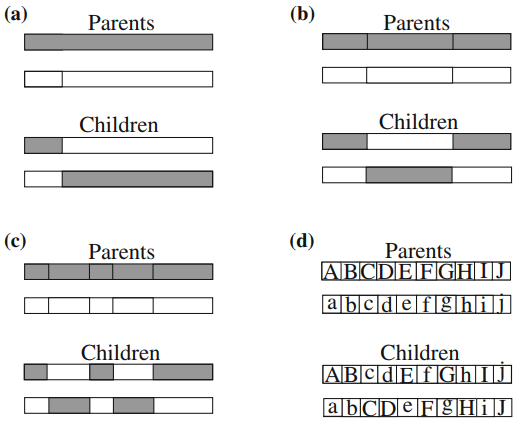
\includegraphics[width=11cm, height=11cm]{cross-over_figure2_1.PNG}
		\end{center}
		
		\noindent \textbf{Figure 2.1} Illustration of crossover operators. \textbf{a} One-point crossover. 
		\textbf{b} Two-point 		crossover. \textbf{c}	Multipoint crossover. \textbf{d} Uniform crossover. For
		multipoint crossover and uniform crossover, the exchange	between crossover	points takes place at a fixed
		probability.
		
			\subsubsection{Multipoint Crossover}Multipoint crossover treats each string as a ring of bits divided by m
			crossover points into m segments, and each segment is exchanged at a fixed probability.
			
			\subsubsection{Uniform Crossover}Uniform crossover exchanges bits of a string rather than segments.
			Individual bits in the parent chromosomes are compared, and each of the nonmatching bits is probabilistically
			swapped with a fixed probability, typically 0.5. The operator is unbiased with respect to defining length. In
			half-uniform crossover, exactly half of the nonmatching bits are swapped. \par
			One-point and two-point	crossover	operations preserve schemata due to low disruption rates. In contrast,
			uniform crossover swaps are more exploratory, but have a high disruptive nature. Uniform crossover is more
			suitable for small populations,	while two-point crossover is better for large populations. Two-point
			crossover performs consistently better than one-point crossover. \par
			When all the chromosomes are very similar or even the same in the population, it is difficult to generate a
			new structure by crossover only and premature convergence takes place. Mutation	operation can introduce
			genetic diversity into the population. This prevents premature convergence from	happening when all the
			individuals in the population become very similar.
			
		\subsection{Mutation}Mutation is a unary operator that requires only one parent to generate an offspring.
		A mutation operator typically selects a random position of a random chromosome and replaces the corresponding
		gene or bit by other information. Mutation helps to regain the lost alleles into the population. \par
		Mutations can be classified into point mutations and large-scale mutations. Point mutations are changes to a
		single position, which can be substitutions, deletions, or insertions of a gene or a bit. Large-scale mutations
		can be similar to the point mutations, but operate in multiple positions simultaneously, or at one point with
		multiple genes or bits, or even on the chromosome scale. Functionally, mutation introduces the necessary amount
		of noise to perform hill-climbing. \par
		Inversion and rearrangement operators are also large-scale mutation operators. Inversion operator picks up a
		portion between two randomly selected positions within a chromosome and then reverses it. Swap is the most
		primitive reordering operator, based on which many new unary operators including inversion can be derived. The
		rearrangement operator reshuffles a portion of a chromosome such that the juxtaposition of the genes or bits is
		changed. Some mutation operations are illustrated in \textbf{Figure 2.2}. \par
		Uniform bit-flip mutation is a popular mutation for binary string representations. It independently changes
		each bit of a chromosome with a probability of p. Typically, p = 1/L for a string of L bits. This in
		expectation changes one bit in each chromosome. The probability distribution of fitness values after the
		operation can be exactly computed as a polynomial in $p$.
		
		
		\begin{center}
				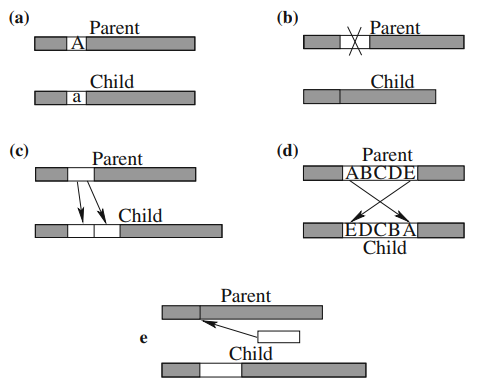
\includegraphics[width=11cm, height=11cm]{mutation_figure2-2.PNG}
		\end{center}
		
		\noindent \textbf{Figure 2.2} Illustration of some mutation operators. \textbf{a} Substitution. 
		\textbf{b} Deletion. \textbf{c} Duplication. \textbf{d} Inversion. \textbf{e} Insertion. \vspace{7mm}
		
		A high mutation rate can lead genetic search to random search. It may change the value of an important bit, and
		thus slow down the fast convergence of a good solution or slow down the process of convergence of the final
		stage of the iterations. In simple GA, mutation is typically selected as a substitution operation that changes
		one random bit in the chromosome at a time. An empirically derived formula that can be used as the probability
		of mutation $P_m$ at a starting point is $p_m = \frac{1}{T \sqrt{l}}$ for a total number of T generations and a
		string length of $l$. \par
		The random nature of mutation and its low probability of occurrence leads to slow convergence of GA. The search
		process can be expedited by using the directed mutation technique [6] that deterministically introduces new
		points into the population by using gradient or extrapolation of the information acquired so far. \par
		It is commonly agreed that crossover plays a more important role if the population size is large, and mutation
		is more important if the population size is small. \par
		In addition to traditional mutation operators, hill-climbing and bit climber are two well-known local search
		operators, which can be treated as mutation operators. Hill-climbing operators find an alternative similar
		individual that represents a local minimum close to the original individual in the solution space. The bit
		climber is a simple stochastic bit-flipping operator. The  fitness is computed for an initial string. A bit of
		the string is randomly selected and flipped, and the fitness is computed at the new point. If the fitness is
		lower	than its earlier value, the new string is updated	as the current string. The operation repeats until no
		bit flip improves the fitness. The bit-based descent algorithm is several times faster than an efficient GA .
		
		\subsection{Exploitation Versus Exploration}For EAs, two fundamental processes that drive the evolution of a
		population are the exploration process and the exploitation process. \textit{Exploitation} means taking
		advantage of the information already obtained, while \textit{exploration} means searching different regions of
		the	search space.	Exploitation is achieved by the selection procedure, while exploration is achieved by genetic
		operators, which preserve genetic diversity in the population. The two objectives are conflicting: increasing
		the selective	pressure leads to decreasing diversity, while keeping the diversity can result in delayed
		convergence. \par
		GA often converges rather prematurely before the optimal solution is found. To prevent premature convergence,
		an appropriate diversity in the population has to be maintained. Otherwise, the entire population tends to be
		very similar, and crossover will be useless and GA reduces to parallel mutation climbing. The trade-off between
		exploitation (convergence) and exploration (diversity) controls the performance of GA and is determined by the
		choice of the control parameters, namely, the probability of crossover $P_c$, the probability of mutation $P_m$
		, and	the population size $N_P$. Some trade-offs are made for selecting the optimal control parameters:
		
		\begin{itemize}
			\item Increasing $P_c$ results in fast exploration at the price of increasing the disruption of good strings.
			\item  Increasing $P_m$ tends to transform genetic search into a random search, while it helps reintroduce lost
			alleles into the population.
			\item Increasing $N_P$ increases the genetic diversity in the population and reduces the probability of
			premature convergence, at the price of an increased time of convergence.
		\end{itemize}
		
		These control parameters depend on one another, and their choices depend on the nature of the problem. In GA
		practice, for small NP one can select relatively large $P_m$ and $P_c$, while for large $N_P$ smaller $P_c$ and
		$P_m$ are desirable. Empirical results show that GA with $N_P$ = 20 – 30, $P_c$ = 0.75 – 0.95, and 
		$P_m$ = 0.005 – 0.01 performs well. When crossover is not used, GA can start with large $P_m$, decreasing toward
		the end of the run. In, the optimal $P_m$ is analytically derived as $P_m$ = 1/L for a string length L. \par
		It is concluded from a systematic benchmark investigation on the seven parameters of GA in that crossovermost
		significantly influenced the success of GA,followed by mutation rate and population size and then by
		rerandomization point and elite strategy. Selection method and the representation precision for numerical
		values had least influence.
			\subsubsection{Adapting Control Parameters}Adaptation of control parameters is necessary for the best search
			process. At the beginning of a search process, GA should have more emphasis on exploration, while at a later
			stage more emphasis should be on exploitation. \par
			Increasing Pm and Pc promotes exploration at the expense of exploitation. A simple method to adapt $P_m$ is
			implemented by linearly decreasing $P_m$ with the number of generations, t. $P_m$ can also be modified by
			
			\begin{equation}
				%\[P_m = \frac{\alpha_0e^-\frac{\gamma_0^t}{2} }{N_p \sqrt{l}}\]
				P_m = \frac{\alpha_0e^-\frac{\gamma_0^t}{2} }{N_p \sqrt{l}}
			\end{equation}
			
			\noindent where the constants \alpha_0 > 0, \gamma_0 ≥ 0, and l is the length of the chromosome. In, 
			\alpha_0 = 1.76 and \gamma = 0. \par
			a fitness-based rule is used to assign mutation and recombination rates, with higher rates being
			assigned to those genotypes that are most different in fitness from the fittest individual in the population.
			This results in a reduced probability of crossover for the best solutions available in an attempt to protect
			them. When all the individuals in the population are very similar, the exploration drive will be lost. Rank
			GA is obtained by assigning the mutation rate through a ranking of the population by fitness. This protects
			only the current maximal fitness found, while the rest perform random walks with different step sizes. The
			worst individuals will undergo the most changes. \par
			Dynamic control of GA parameters can be based on fuzzy logic techniques. In, the population sizes, and
			crossover and mutation rates are determined from average and maximum fitness values and differentials of the
			fitness value by fuzzy reasoning.
			
			\subsubsection{Controlling Diversity}The genetic diversity of the population can be easily improved so as to
			prevent premature convergence by adapting the size of the population [1,34] and using partial restart.
			Partial restart is a simple approach to maintain genetic diversity. It can be implemented by a fixed restart
			schedule at a fixed number of generations, or implemented when premature convergence occurs. \par
			Periodic population reinitialization can increase the diversity of the population. One methodology combining
			the effects of the two strategies is saw-tooth GA, which follows a saw-tooth population scheme with a
			specific amplitude and period of variation. \par
			Duplicate removal can enhance the diversity substantially. The uniqueness operator [63] allows a child to be
			inserted into the population only if its Hamming distance to all members of the population is greater than a
			threshold. Analysis of an EA with $N_P > 1$ using uniform bit mutation but no crossover shows that the
			duplicate removal method changes the time complexity of optimizing a plateau function from exponential to
			polynomial. Each child is required to compare with all the solutions in the current population. \par
			Diversity-guided EA uses the distance-to-average-point measure to alternate between phases of
			exploration (mutation) and phases of exploitation (recombination and selection). The diversity-guided EA has
			shown remarkable results not only in terms of fitness, but also in terms of saving a substantial amount of
			fitness evaluations compared to simple EA. \par
			Since the selection operator has a tendency to reduce the population variance, population variance can be
			increased by the variation operator to maintain adequate diversity in the population. A variation operator
			is a combination of the recombination and the mutation operator. For a variation operator, population mean
			decision variable vector should remain the same before and after the variation operator.
			
			\subsubsection{Varying Population Size}Population sizing schemes for EAs may rely on the population sizing
			theory, or include the concepts of age, lifetime, and competition among species for limited resources. In, a
			thorough analysis of the role of the offspring population size in an EA is presented using a simplified, but
			still realistic EA. The result suggests a simple way to dynamically adapt this parameter when necessary. \par
			MessyGA startswith a large initial population and halves it atregular intervals during the primordial stage.
			In the primordial stage only a selection operation is applied. This helps the population to get enriched with
			good building blocks. Fast messy GA is an improved version of messy GA. \par
			GENITOR employs an elitist selection that is a deterministic, rank-based selection method so that the
			best $N_P$ individuals found so far are preserved by using a crossgenerational competition. Crossover
			produces only one offspring that immediately enters the population. Offspring do not replace their parents,
			except for those least-fit individuals in the population. This selection strategy is similar to the
			$(\lambda + \mu)$ strategy of ES. \par
			CHC algorithm stands for crossgenerational elitist selection, heterogeneous recombination, and
			cataclysmic mutation. Like GENITOR, it also borrows from the $(\lambda + \mu)$ strategy of ES. Incest
			prevention is introduced so that similar individuals are prevented from mating. Half-uniform crossover is
			applied, and mutation is not performed. Diversity is reintroduced by restarting partial population whenever
			convergence is detected. This is implemented by randomly flipping a fixed proportion of the best individual
			found so far as template, and introducing the better offspring into the population. \par
			Parameterless population pyramid is an efficient, general, parameterless evolutionary approach without
			user-specified parameters. It replaces the generational model with a pyramid of multiple populations that are
			iteratively created and expanded. The approach scales to the difficulty of the problem when combined with
			local search, advanced crossover, and addition of diversity.
			
			\subsubsection{Aging}Aging provides a mechanism to make room for the development of the next generation.
			Aging is a general mechanism to increase genetic diversity. An optimal lifespan plays an important role in
			improving the effectiveness of evolution. For intelligent species which are able to learn from experience,
			aging avoids excessive experience accumulation of older individuals to avoid their being always the superior
			competitors. \par
			Aging is often used by assigning age 0 to each new offspring. The age is increased by 1in each generation. In
			selection for replacement the age is taken into account: Search points exceeding a predefined maximal age are
			removed from the collection of search points. \par
			In cohort GA, a string of high fitness produces offspring quickly, while a string of low fitness may
			have to wait a long time before reproducing. All strings can have the same number of offspring, say two, at
			the time they reproduce. To implement this delayed-reproduction idea, the population of cohort GA is divided
			into an ordered set of nonoverlapping subpopulations called cohorts. Reproduction is carried out by cycling
			through the cohorts in the given order.
			
			\begin{center}
				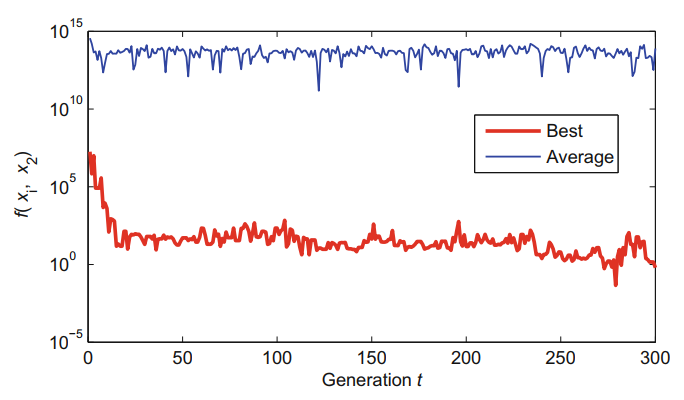
\includegraphics[width=11cm, height=7cm]{exploitation-vs-exploration_figure-2-3.PNG}
			\end{center}
			
			\noindent \textbf{Figure 2.3} The evolution of a random run of simple GA: the maximum and average objectives.
			
		\section{Numerical Methods}
		\textbf{Example 3.1}: The conversion from binary coding to Gray coding is formulated as
		\begin{center}
		\[
			$g_i$ = 
			\begin{cases}
				$b_1$,                 & \text{$i = 1$} \\
				$b_i$\oplus $b_{i-1},  & \text{$i > 1$}
			\end{cases}
		\]$
		\end{center}
		where $g_i$ and $b_i$ are, respectively, the $i$th Gray code bit and the $i$th binary code bit, which are
		numbered from 1	to n starting on the left, and $\oplus$ denotes addition mod 2, i.e., exclusive-or. Gray coding
		can be converted into	binary coding by where $g_i$ and bi are, respectively, the $i$th Gray code bit and the 
		$i$th	binary code bit, which are numbered from 1 to n starting on the left, and $\oplus$ denotes addition mod 2,	i.e.,	exclusive-or. Gray coding can be converted into binary coding by
		\begin{center}
		\[
			$b_i$ = \sum_{j=1}^{i}
		\]
		\end{center}
		where the summation denotes summation mod 2. As an example, we can check the equivalence between the binary
		code 1011011011 and the gray code 1110110110. From the two equations, the most significant i bits of the binary
		code determine the most significant i bits of the Gray code and vice versa. \vspace{2mm}
		
		\noindent \textbf{Example 3.2}:In this example, we apply simple GA to solve optimization of Rosenbrock function
		plotted in Example 1.1. The domain is x1, x2 ∈ [−2048, 2048]. For simple GA without elite strategy, the size of
		population is 100, and the representation for each variable is 30-bit Gray coding. Single-point crossover with
		Pc = 0.98 is applied, and Pm = 0.02. The selection scheme is the roulette-wheel
		selection. In each generation, 90 \% of the population is newly generated. The evolution for 300 generations for
		a typical random run is shown in Figure 3.4. At the end of the 300th generation, the best solution is x1 = 1
		4171, x2 = 1.9413, and f = 0.6198. The best solution is present at the end of the 279th generation, x1 = 0.8060
		, x2 = 0.6409, and f = 0.6198. The global minimum is $f^ \ast$ = 0 at x1 = 1, x2 = 1. \vspace{2mm}
		
		\noindent \textbf{Example 3.3}:  In this example, we solve optimization of Rosenbrock function given in 
		Example 1.1 by using real-coded GA. The domain is x1, x2 ∈ [−2, 048, 2, 048]. The global optimum fitness is 
		0 at (1, 1).
		For most numerical optimization problems, real coding can usually generate a performance better than that of
		binary coding. Here we include the elitism strategy in the real-coded GA realization. Our numerical test shows
		that a high mutation rate can usually yield good results. We select $N_P$ = 100, $P_c$ = 0.9, $P_m$ = 0.9.
		Roulettewheel selection scheme is adopted. The crossover operator generates, by averaging two parents, only one
		offspring. One point mutation is employed. The mutation operator rejects infeasible chromosomes that are beyond
		the domain. An annealing variance $\sigma = \sigma_0(1 − \frac{1}{T} ) + \sigma_1$ is selected for Gaussian
		mutation, where $\sigma_0 = 30$, and $\sigma_1 = 0.1$, and t corresponds to the number of generations. Except for
		the largest chromosome of the old generation, all chromosomes in the old generations are replaced by the new
		offspring. \par
		The evolution for T = 300 generations for a typical random run is shown in Figure 3.1. At the end of the 300th
		generation, the solution of a typical run is $x_1 = 0.9338$, $x_2 = 0.8719$, and $f = 0.0044$. The adaptation
		is shown in Figure 3.1. Realcoded GA typically leads to a performance better than that of simple GA based on
		a random run.
		
		\begin{center}
				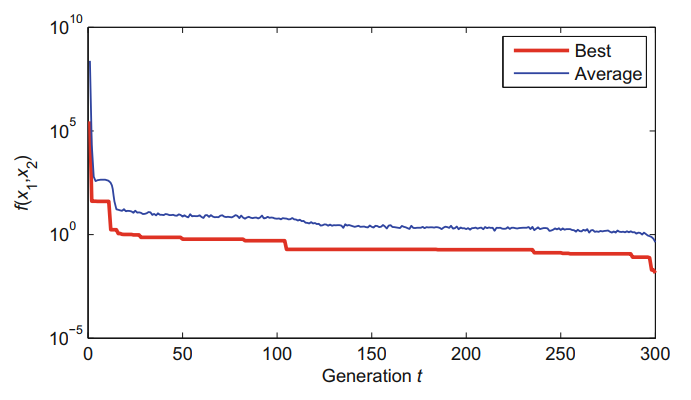
\includegraphics[width=11cm, height=9cm]{figure_3-1.PNG}
		\end{center}
		
		\noindent \textbf{Figure 3.1} The evolution of a random run of the real-coded GA with the elitism strategy: the
		maximum and average objectives.
		
	  \section{Conclusion}In genetics, a strong distinction is drawn between the genotype and the phenotype; the
		former contains genetic information, whereas the latter is the physical manifestation of this information. Both
		play a role in evolution as the biological processes of diversity generation act on the genotype, while the
		‘worth’ or fitness of this genotype in the environment depends on the survival and reproductive success of its
		corresponding phenotype. Similarly, in the canonical GA a distinction is made between the encoding of a
		solution (the ‘genotype’), to which simulated genetic operators are applied, and the phenotype associated with
		that encoding. These phenotypes can have many diverse forms depending on the application of interest. Unlike
		traditional optimisation techniques the GA maintains and iteratively improves a population of solution
		encodings. Evolutionary algorithms, including the GA, can be broadly characterised as 
		\[x[t + 1] = r(v(s(x[t])))\]
		where $x[t]$ is the population of encodings at timestep $t$, $v(.)$ is the random variation operator (crossover
		and mutation), $s(.)$ is the selection for mating operator, and $r(.)$ is the replacement selection operator. 
		
		\begin{center}
				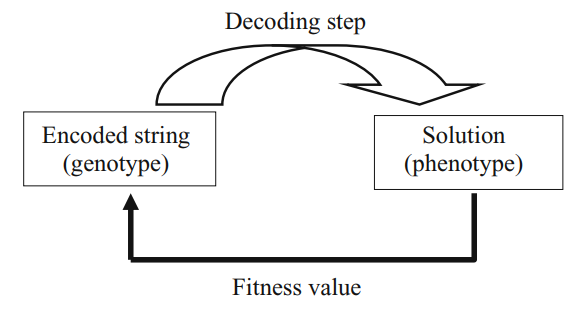
\includegraphics[width=11cm, height=7cm]{figure_4-1.PNG}
		\end{center}
		
		\noindent \textbf{Fig. 4.1}.Decoding of genotype into a solution in order to calculate fitness
	
		
		\section{References}
		\begin{enumerate}
			\item Ke-Lin Du • M.N.S. \textbf{Swamy Search and Optimization by Metaheuristics} Techniques and Algorithms
			Inspired by Nature
			\item Anthony Brabazon • Michael O’Neill Seán McGarraghy \textbf{Natural Computing Algorithms}
			\item Arabas J, Michalewicz Z, Mulawka J. GAVaPS—a genetic algorithm with varying population size. In:
			Proceedings of the 1st IEEE international conference on evolutionary computation, Orlando, FL, USA, 
			June 1994. p. 73–78.
			\item Araujo L, Merelo JJ. Diversity through multiculturality: assessing migrant choice policies in
			an island model. IEEE Trans Evol Comput. 2011;15(4):456–69.
			\item Ballester PJ, Carter JN. An effective real-parameter genetic algorithm with parent centric normal
			crossover for multimodal optimisation. In: Proceedings of genetic and evolutionary computation conference 
			(GECCO), Seattle, WA, USA, June 2004. p. 901–913.
		\end{enumerate}
	
		
\end{document}

